%%%%%%%%%%%%%%%%%%%%%%%%%%%%%%%%%%%%%%%%%%%%%%%%%%%%%%%%%%%%%%%%%%%%%%%%%%%%%%%%%%%%%%%
%%%%%%%%%%%%%%%%%%%%%%%%%%%%%%%%%%%%%%%%%%%%%%%%%%%%%%%%%%%%%%%%%%%%%%%%%%%%%%%%%%%%%%%
% 
% This top part of the document is called the 'preamble'.  Modify it with caution!
%
% The real document starts below where it says 'The main document starts here'.


\documentclass[12pt]{article}

\usepackage{amssymb,amsmath,amsthm}
\usepackage[top=1in, bottom=1in, left=1.25in, right=1.25in]{geometry}
\usepackage{fancyhdr}
\usepackage{listings}
\usepackage{enumerate}
\usepackage{hieroglf}
\usepackage{oands}
\usepackage{arevmath}
\usepackage{relsize}
\usepackage{times,txfonts}
\usepackage{graphicx}
\usepackage{float}

\newtheoremstyle{homework}% name of the style to be used
  {18pt}% measure of space to leave above the theorem. E.g.: 3pt
  {12pt}% measure of space to leave below the theorem. E.g.: 3pt
  {}% name of font to use in the body of the theorem
  {}% measure of space to indent
  {\bfseries}% name of head font
  {:}% punctuation between head and body
  {2ex}% space after theorem head; " " = normal interword space
  {}% Manually specify head
\theoremstyle{homework} 

% Set up an Exercise environment and a Solution label.
\newtheorem*{exercisecore}{Exercise \@currentlabel}
\newenvironment{exercise}[1]
{\def\@currentlabel{#1}\exercisecore}
{\endexercisecore}

\newcommand{\localhead}[1]{\par\smallskip\noindent\textbf{#1}\nobreak\\}%
\newcommand\solution{\localhead{Solution:}}

%%%%%%%%%%%%%%%%%%%%%%%%%%%%%%%%%%%%%%%%%%%%%%%%%%%%%%%%%%%%%%%%%%%%%%%%
%
% Stuff for getting the name/document date/title across the header
\makeatletter
\RequirePackage{fancyhdr}
\pagestyle{fancy}
\fancyfoot[C]{\ifnum \value{page} > 1\relax\thepage\fi}
\fancyhead[L]{\ifx\@doclabel\@empty\else\@doclabel\fi}
\fancyhead[C]{\ifx\@docdate\@empty\else\@docdate\fi}
\fancyhead[R]{\ifx\@docauthor\@empty\else\@docauthor\fi}
\headheight 15pt

\def\doclabel#1{\gdef\@doclabel{#1}}
\doclabel{Use {\tt\textbackslash doclabel\{MY LABEL\}}.}
\def\docdate#1{\gdef\@docdate{#1}}
\docdate{Use {\tt\textbackslash docdate\{MY DATE\}}.}
\def\docauthor#1{\gdef\@docauthor{#1}}
\docauthor{Use {\tt\textbackslash docauthor\{MY NAME\}}.}
\makeatother

% Shortcuts for blackboard bold number sets (reals, integers, etc.)
\newcommand{\Reals}{\ensuremath{\mathbb R}}
\newcommand{\Nats}{\ensuremath{\mathbb N}}
\newcommand{\Ints}{\ensuremath{\mathbb Z}}
\newcommand{\Rats}{\ensuremath{\mathbb Q}}
\newcommand{\Cplx}{\ensuremath{\mathbb C}}
%% Some equivalents that some people may prefer.
\let\RR\Reals
\let\NN\Nats
\let\II\Ints
\let\CC\Cplx

%%%%%%%%%%%%%%%%%%%%%%%%%%%%%%%%%%%%%%%%%%%%%%%%%%%%%%%%%%%%%%%%%%%%%%%%%%%%%%%%%%%%%%%
%%%%%%%%%%%%%%%%%%%%%%%%%%%%%%%%%%%%%%%%%%%%%%%%%%%%%%%%%%%%%%%%%%%%%%%%%%%%%%%%%%%%%%%
% 
% The main document start here.

% The following commands set up the material that appears in the header.
\doclabel{Math 316: HW 2}
\docauthor{Stefano Fochesatto}
\docdate{\today}

\begin{document}


\textbf{Section 2.5}
\begin{enumerate}
\item Write the fraction $\frac{5}{3}$ in sexagesimal notation by
\begin{enumerate}
\item using the Babylonian method of finding the reciprocal of the denominator and then multiplying by the numerator.\\
\end{enumerate}

\textbf{Answer:} First we must find the reciprocal of 3. In sexagesimal notation we need some $x$ that gives us,
\begin{equation*}
  3x = y
\end{equation*}
Where $y$ is some power of 60. Written in sexagesimal $y$ would look like $1,0;$ or $0;1$. through the doubling multiplication table we can find
such a $y$. Consider the doubling table starting with 3,
\begin{align*}
  1 &| 3\\
  2 &| 6\\
  *4 &| 12\\
  8 &| 24 \\
  *16 &| 48\\
\end{align*} 
Now note that, $12 + 48 = 1,0;$ and therefore we know that $3*(16+4) = 1,0;$. In order to turn the right hand side of the equation into $1$ and find the true reciprocal
we want to divide by $60$ or $1,0;$ and the babylonians did this by simply shifting the digits similarly to how we divide by powers of 10. Thus we get that the reciprocal of 3 is 
$;20$. Now we want to find the product $5 *;20$ we can do this through the doubling table,
\begin{align*}
  *1 &| ;20\\
  2 &| ;40\\
  *4 &| 1;20\\
\end{align*}
Finally we get that $5*;20 = 1;40$.
\vspace{.5in}



\setcounter{enumi}{3}
\item A typical Babylonian problem of $1700$ B.C. calls for finding the sides of a rectangle given its semi-perimeter and area; that is, solve systems of equations of the type $x+y=a$, $xy=b$. Find the solution of the particular system $x+y=10$, $xy=16$. [Hint: The Babylonians might have used the identity $(x-y)^2=(x+y)^2-4xy$ to find $x-y$.]\\

\textbf{Answer:} Substituting our given values of $x + y = 10$ and $xy = 16$ into the the identity $(x-y)^2 = (x+y)^2 - 4xy$ we get the following,
\begin{equation*}
  (x-y)^2 = (10)^2 - 4(16) = 1,40 - 1,4 = 36
\end{equation*}
Therefore we know that $x - y = 6$. then the Babylonians would have solved the following system, 
\begin{equation*}
  x - y = 6, 
\end{equation*}
\begin{equation*}
  xy = 16
\end{equation*}
by first calculating $\frac{6}{2} = 3$ then applying a formula, where
\begin{equation*}
  x = z + 3
\end{equation*}
\begin{equation*}
  y = z - 3
\end{equation*}
We can quickly solve for $z$ however the texts states that the Babylonians had a formula where $z = \sqrt{(\frac{a}{2})^2 - b}$. Using $x + y = 10$
we get that (Note: they could have also seen this),
\begin{align*}
  (z + 3) + (z - 3) = 10\\
  2z = 10\\
  z = 5
\end{align*}
Finally substituting $z = 5$ and gives us $x = 8$ and $y = 2$.
\vspace{.5in}



\item Another Babylonian problem is,
\begin{center}
To the area of a rectangle, the excess of the length over the width is added, giving 120; moreover, the sum of the length and width is 24. Find the dimensions of the rectangle.
\end{center}
[Hint: The problem can be put in the form of two equations $xy+x-y=120$, $x+y=24$; if the substitution $y=z-2$ is made, the system becomes $x+z=26$, $xz=144$.]\\

\textbf{Answer:} The babylonians would often reduce bigger algebra problems into ones similar to the last problem. By setting $y = z-2$ we get a 
similar reduction. Substitution into the second equation get us,
\begin{align*}
  x + (z - 2) &= 24,\\
  x + z &= 26,
\end{align*} 
Simplifying the second equation after requires 2 substitution,
\begin{align*}
  x(z-2)+x-(z - 2)&=120,\\
  xz-2x + x - z +2 &=120,\\
  xz - x - z + 2 &=120,\\
  xz - x - z &=118,\\
  xz - (x + z) &=118,\\
  xz - 26 &=118,\\
  xz &=144.\\
\end{align*}
The text gives this as the result as well however I'm skeptical that the Babylonians would have been able to get to it using the algebra from above. 
Now using the previous identity we will solve for $x-z$, 
\begin{equation*}
  (x-z)^2 = (26)^2 - 4(144) = 100.
\end{equation*}
Therefore we get that $x - z = 10$. Setting $x = q + \frac{10}{2}$ and $z = q - \frac{10}{2}$ we solve for $q$ using $x + z = 26$,
\begin{align*}
  (q - 5) + (q + 5) &= 26,\\
  2q &= 26,\\
  q &= 13.
\end{align*}
Thus we get that $x = 18$ and $z = 8$ and therefore $y = 6$.
\vspace{.5in}

\setcounter{enumi}{8}
\item A classical example of the quadratic equation in Babylonian mathematics is found on a tablet in the British Museum, which states:
\begin{center}
I have added 7 times the side of my square to 11 times its surface to obtain 6;15. Reckon with 7 and 11.
\end{center}
Solve for the scribe’s answer of 0;30 for the side of the square. [Hint:  The injunction to “reckon with 7 and 11” means simply that $11x^2+7x=6;15$. Multiply both sides of this equation by 11 thereby turning it into a quadratic in $11x$.]\\

\textbf{Answer:} It is discussed in the text that the Babylonians actually had a formula for solving quadratic equations of the form,
\begin{equation*}
  x^2 +ax = b
\end{equation*}
With the following formula,
\begin{equation*}
  x = \sqrt{(\frac{a}{2})^2 + b} - \frac{a}{2}.
\end{equation*}
The hint suggests performing a substitution and multiplying both sides of the equation by 11. Showing how this formula was derived geometrically and 
also solving for $x$ we get,
\begin{center}
  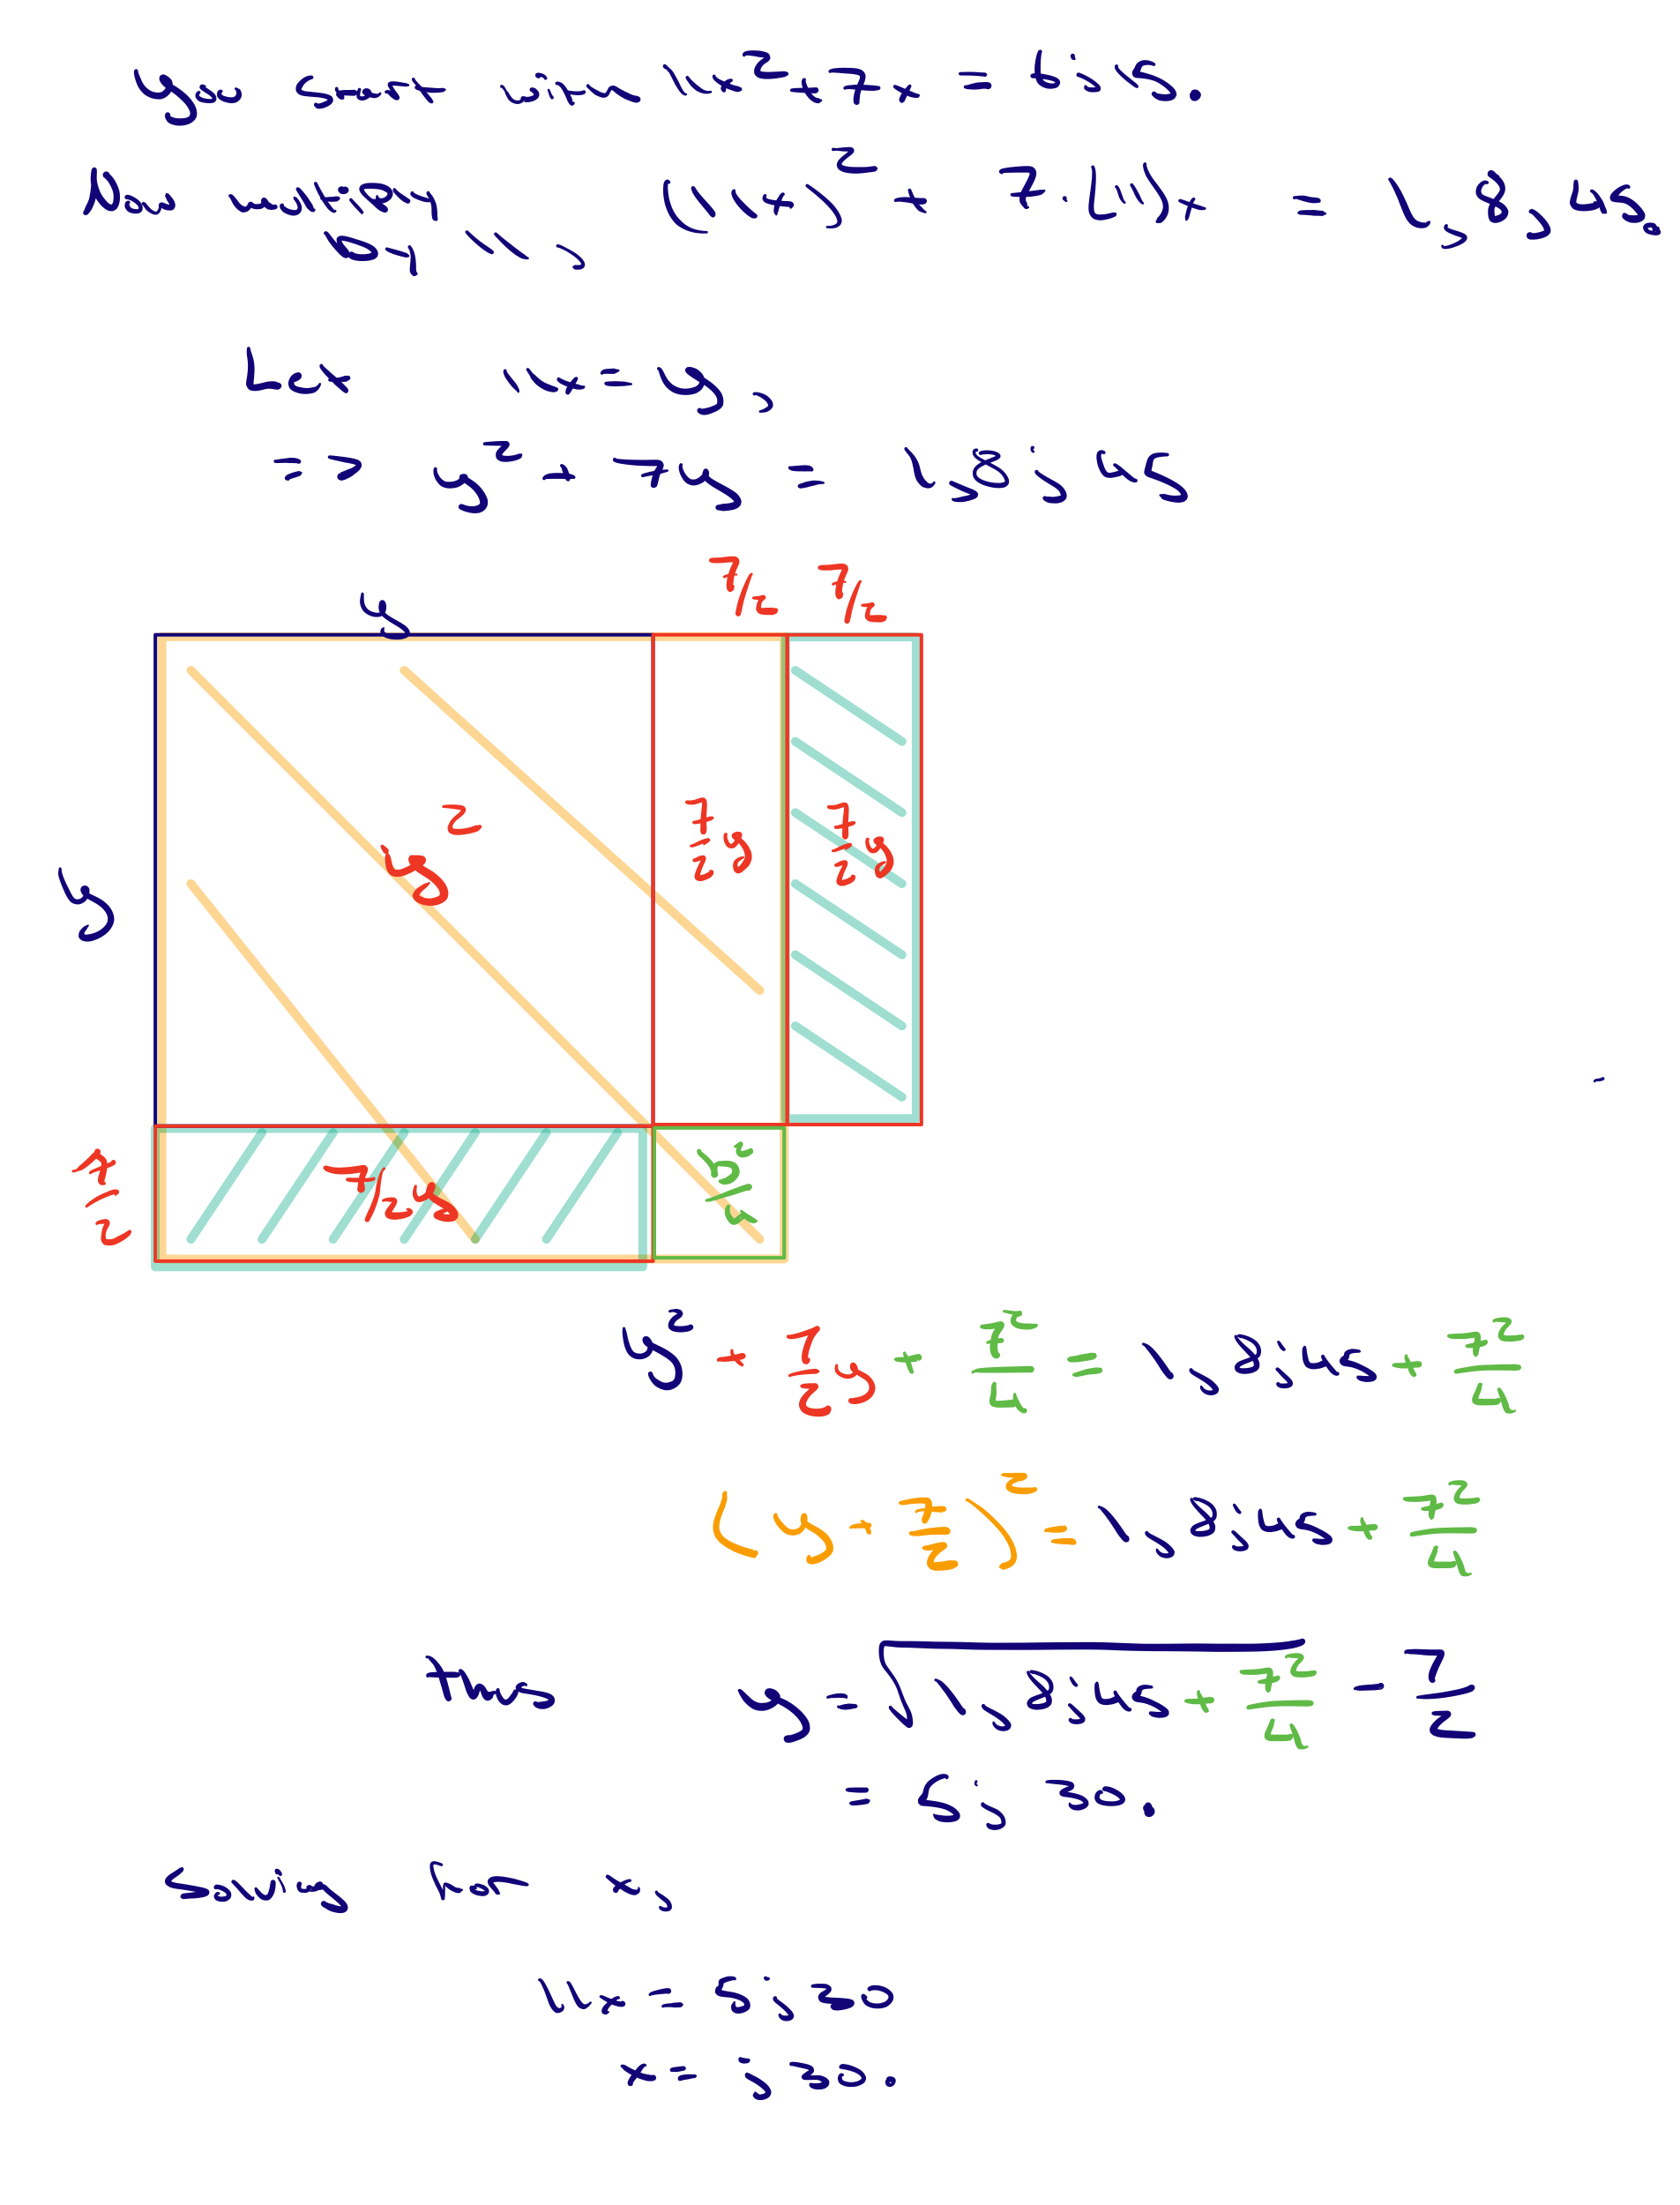
\includegraphics[width = .75\textwidth]{square.png}        
\end{center}

\vspace{.5in}
\end{enumerate}
\vspace{.5in}





\textbf{Section 2.6}
\begin{enumerate}
\setcounter{enumi}{6}
\item Because $a$ is smaller than $\sqrt{a^2+b}$ when $b>0$ whereas $a+b/a$ is larger, the Babylonian mathematician often approximated $\sqrt{a^2+b}$ by taking the average of these two values; that is,
\begin{align*}
\sqrt{a^2+b}&\approx\frac{1}{2}\left[a+\left(a+\frac{b}{a}\right)\right]\\
&=a +\frac{b}{2a} &0<b<a^2
\end{align*}
Use this formula to get a rational approximation to $\sqrt{17}$. [Hint: In the first case put $a=\frac{4}{3},$ $b=\frac{2}{9}$. In the second case put $a=2$, $b=1$.]\\

\textbf{Answer:} To find the rational approximation of $\sqrt{17}$ first we need to find a suitable $a$ and $b$ such that $0 < b < a^2$ and,
\begin{equation*}
  a^2 + b = 17. 
\end{equation*}
Lets set $a = 4$ and $b = 1$. Applying the Babylonian algorithm,
\begin{equation*}
  \sqrt{4^2 + 1} \approx \frac{1}{2} [a + (a + \frac{b}{a})].
\end{equation*}
\begin{equation*}
  \sqrt{17} \approx ;30 [4 + (4 + ;15)] = ;30(8;15) = 4;7,30
\end{equation*}
\end{enumerate}

\vspace{.5in}





\textbf{Section 3.2}
\begin{enumerate}
\item Plutarch (about A.D. 100) stated that if a triangular number is multiplied by 8, and 1 is added, then the result is a square number. Prove that this is fact and illustrate it geometrically in the case of $t_2$.\\

\textbf{Answer:} this result can be proven multiple ways. First I will demonstrate that it is true with modern notation. Recall that a triangular number $t_n$ can be calculated using the following equation,
\begin{equation*}
  t_n = \frac{n(n+1)}{2}.
\end{equation*}
To prove this result we need to see if the expression $8(t_n) +1$ produces a perfect square. Substituting our function for $t_n$,
\begin{align*}
  8(t_n)+1 &= 8\frac{n(n+1)}{2} + 1,\\
  &= 4n(n+1) + 1,\\
  &= 4n^2 + 4n + 1,\\
  &= (2n + 1)^2.
\end{align*}
As we can see Plutarch's claim is true and will always result in an odd sized square number. This will allow us to prove this proposition with a picture. Note that
for an odd sized square number there will always be a center point. That center point will always be surrounded by 8 points. Fill in the center point to account for the $+1$ then 
each of the 8 surrounding points will correspond one to one with the 8 triangles. This is shown with the right most $s_5$ square and is composed of $t_2$ triangles. 
\begin{center}
  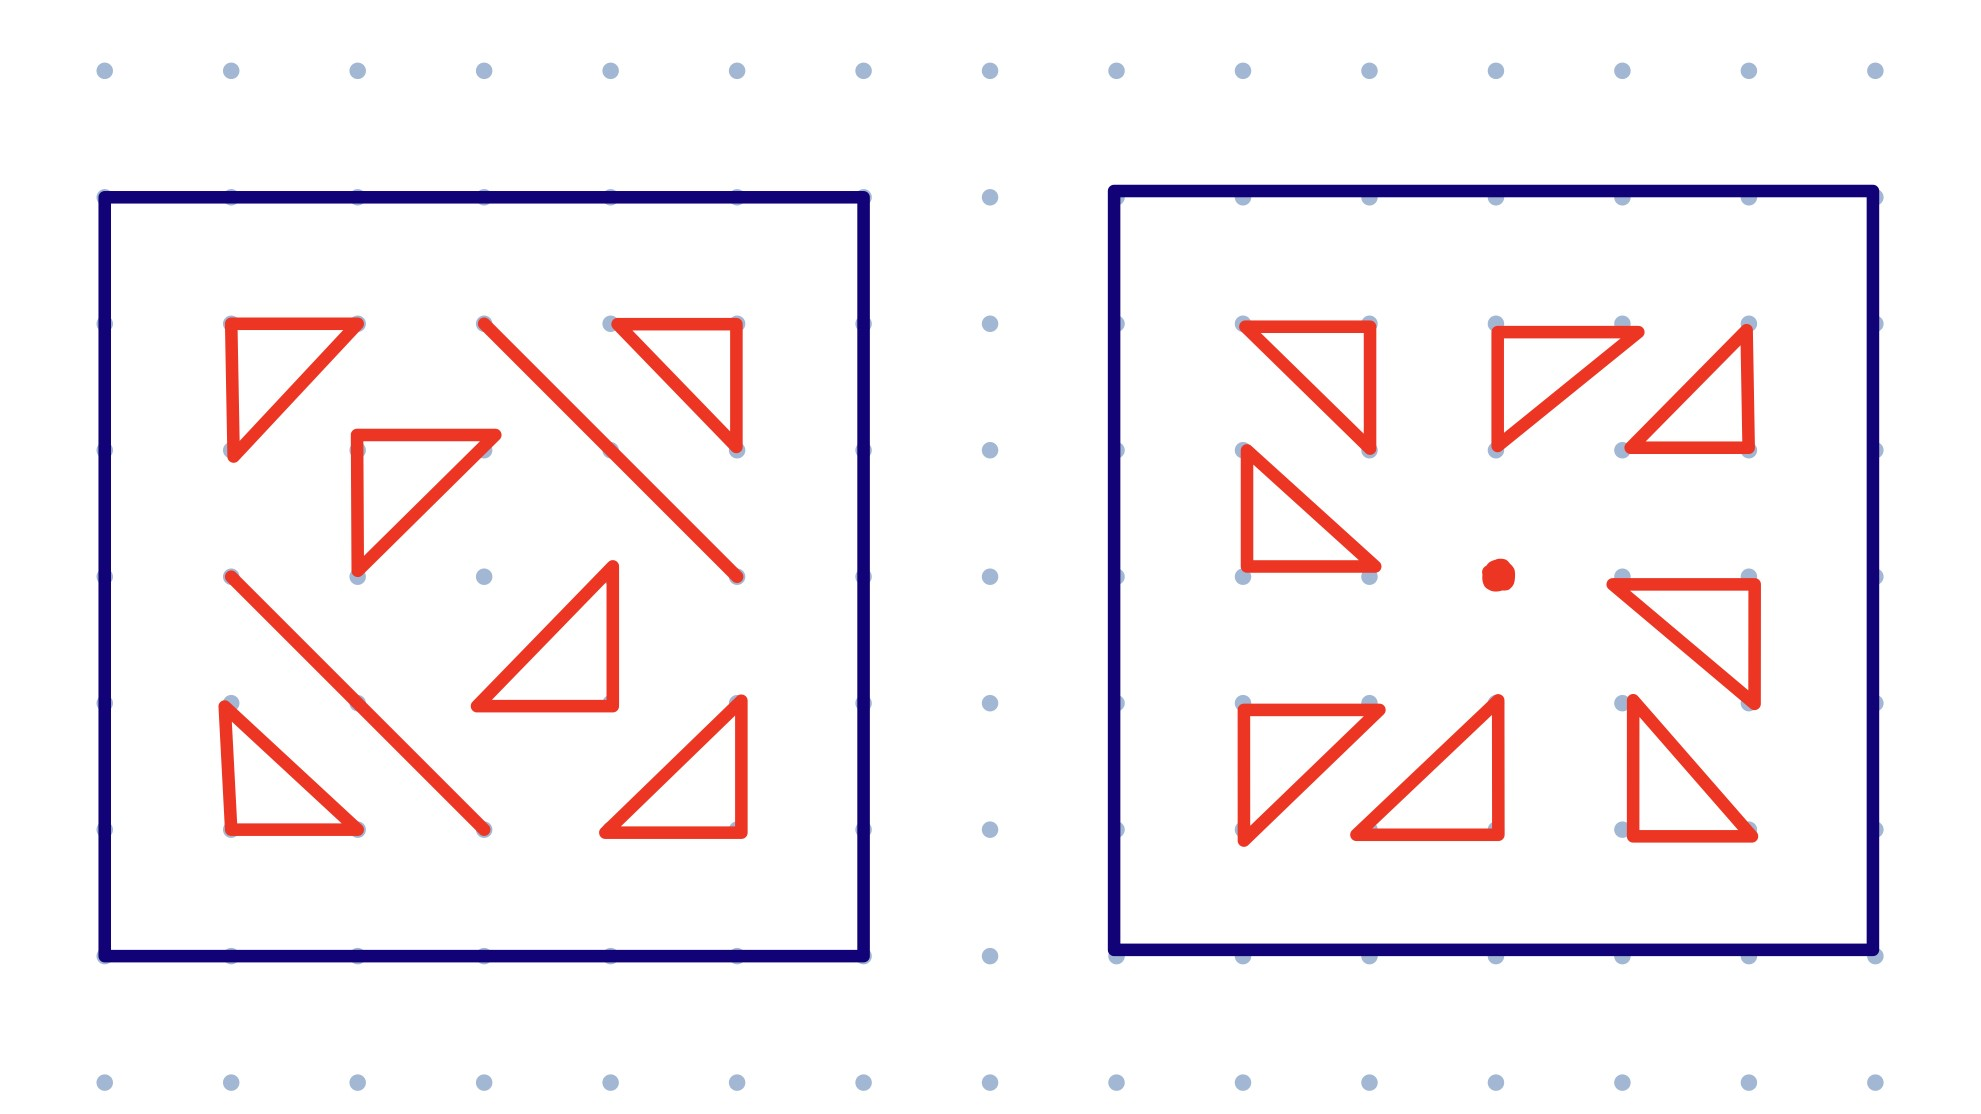
\includegraphics[width = .75\textwidth]{squares.jpg}        
\end{center}




\vspace{.5in}
\setcounter{enumi}{6}
\item An oblong number counts the number of dots in a rectangular array having one more row than it has columns; the first few of these numbers are, $2,6,12,20$ and in general, the $n$-th oblong number is given by $o_n=n(n+1)$. Prove algebraically and geometrically that,
\begin{enumerate}
\setcounter{enumii}{1}
\item Any oblong number is the sum of two equal triangular numbers.\\
\end{enumerate}

\textbf{Answer:} Simply recall that the text proves that,
  \begin{equation*}
    t_n = \frac{n(n+1)}{2}.
  \end{equation*}
Therefore by substitution into the oblong-number function we get that, $0_n = 2t_n$. Pictorially any $o_n$ can be bisected along the 
diagonal to show that it is composed of two equal triangles. 
  \begin{figure}[H]
    \begin{center}
    \caption{An $o_4$ bisected into 2 $t_4$}
  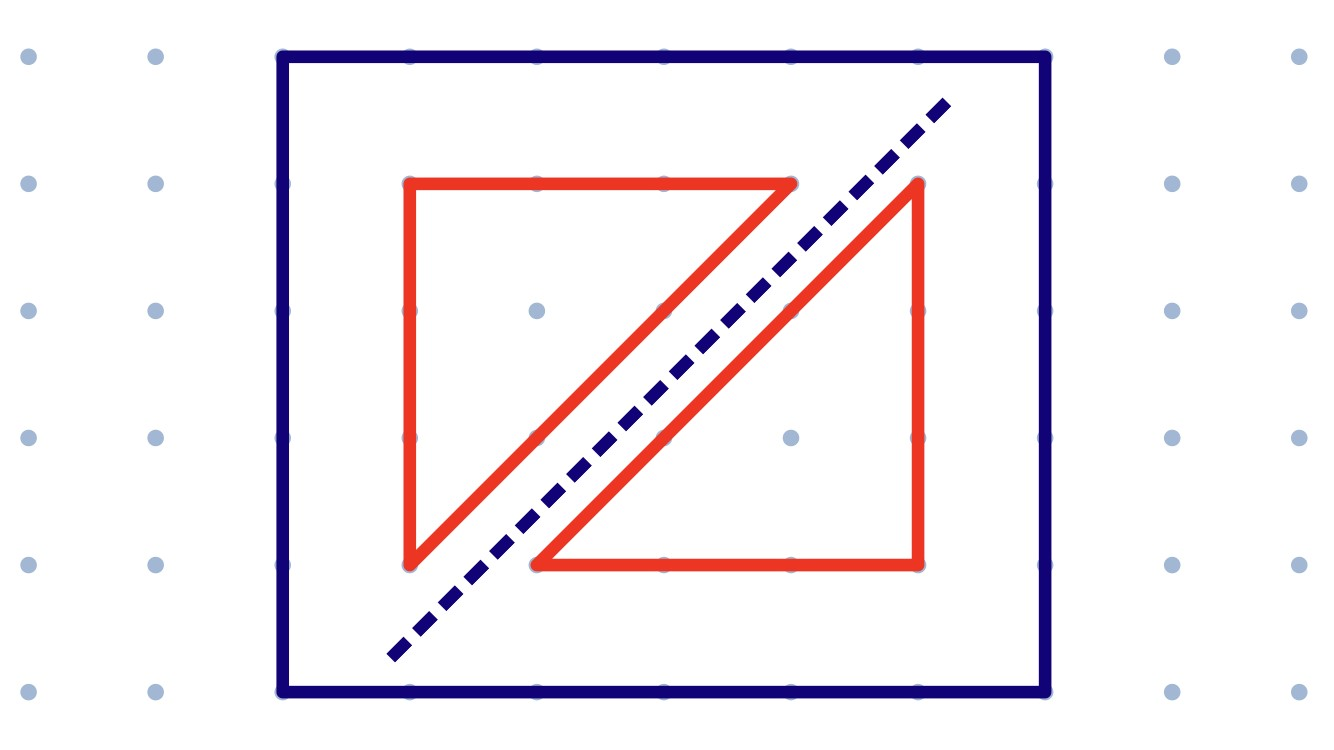
\includegraphics[width = .50\textwidth]{oblong.jpg}      
\end{center}
\end{figure}



\end{enumerate}
\vspace{.5in}





\textbf{Section 3.3}
\begin{enumerate}
\setcounter{enumi}{1}
\item Find all the right triangles with sides of integral length whose areas are equal to their perimeters. [Hint: The equations $x^2 + y^2 = z^2$
and $x + y + z = \frac{1}{2}xy$ imply that $(x-4)(y - 4) = 8$.]\\

\textbf{Answer:}To prove this with modern methods all we have to do is solve the system of linear equations. First we take the second equation and solve for $z$,
\begin{equation*}
  z = x + y - \frac{1}{2}xy.
\end{equation*} 
Now we want to square $z$ and expand the terms,
\begin{equation*}
  z^2 = \frac{1}{4}x^2y^2 -x^2y - xy^2 + 2xy + x^2 + y^2.
\end{equation*}
Substituting our value of $z^2$ into the pythagorean theorem and subtracting $x^2 + y^2$ from both sides,
\begin{equation*}
  0 = \frac{1}{4}x^2y^2 -x^2y - xy^2 + 2xy.
\end{equation*}
With some algebra we get that, 
\begin{align*}
  0 &= \frac{1}{4}x^2y^2 -x^2y - xy^2 + 2xy,\\
  -2xy &= \frac{1}{4}x^2y^2 -x^2y - xy^2,\\
  -1 &= \frac{1}{8}xy - \frac{1}{2}x - \frac{1}{2}y,\\
  -8 &= xy - 4x - 4y,\\
  8 &= xy - 4x - 4y + 16,\\
  8 &= (x-4)(y - 4).\\
\end{align*}
Listing the natural factors of 8 we get that, ${(1,8),(2,4)}$ then solving for pairs that satisfy. The first triangle has lengths $5, 12,13 $ and the second triangle has lengths $6, 8, 10$. We solved
for the third length with the pythagorean equation, though they are popular triples.  


\vspace{.5in}





\setcounter{enumi}{3}
\item Verify that $(3,4,5)$ is the only pythagorean triple involving consecutive positive integers. [Hint: Consider the Pythagorean triple $(x, x+1, x+2)$ and show that $x = 3$] \\

\textbf{Answer:} Consider the following pythagorean triple, $(x, x+1, x+2)$. Using the pythagorean equation to solve for $x$ we get,
\begin{align*}
  x^2 + (x+1)^2 &= (x+2)^2,\\
  x^2 + x^2 + 2x +1 &= x^2 + 4x + 4,\\
  x^2  -2x - 3 &=0,\\
  (x-3)(x+1) &=0.\\
\end{align*}
So our solutions are $x = 3, -1$. Given the context of a triangle with positive length, $(3,4,5)$ must be the only consecutive triple.

\vspace{.5in}




\setcounter{enumi}{14}
\item A standard proof of the Pythagorean Theorem starts with a right triangle $ABC$, with its right angles at $C$,
and then draws a perpendicular $CD$ from $C$ to the hypotenuse $AB$. \\
\begin{enumerate}
  \item Prove that triangle $ACD$ and $CBD$ are both similar to triangle $ABC$.\\

  \textbf{Answer:} First note that $\angle CDA = \angle CDB = 90$. Now consider a line $AE$ parallel to $CE$.
 \begin{center}
  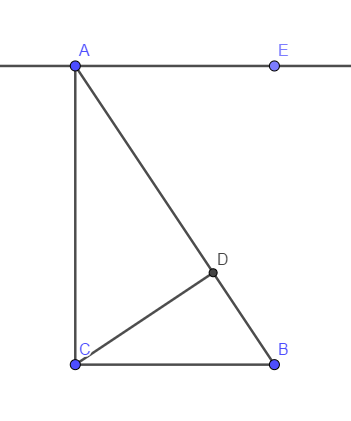
\includegraphics[width = .50\textwidth]{triangle.png}      
   \end{center}
  By Construction we know that $\angle CBD = \angle DAE$. Now consider the following equation for the sum of the angles of triangle $CBD$,
  \begin{equation*}
    90 + \angle CBD + \angle DCB = 180. 
  \end{equation*}
  Now consider the sum of the angles along the line $AE$,
  \begin{equation*}
    90 + \angle DAE + \angle CAD = 180. 
  \end{equation*}
  Since $\angle CBD = \angle DAE$ it must follow that $\angle DCB = \angle CAD$. Thus triangles $ACD$ and $CBD$ are similar by AA similarity.
  Since all triangles are right triangles and each smaller triangle contains an angle from the larger triangle,  triangle $ACD$ and $CBD$ are both similar to triangle $ABC$ by AA similarity.
  \vspace{.5in}


  \item For triangle $ABC$ with legs of lengths $a$ and $b$ and with a hypotenuse of length $c$, use proportionality of corresponding sides of similar triangles to
  establish the Pythagorean theorem.\\

  \textbf{Answer:} Let $a = AC$, $b = BC$, and $c = AB$. 
  \begin{center}
    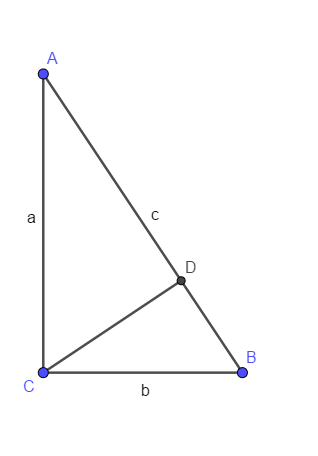
\includegraphics[width = .50\textwidth]{triangle2.png}      
     \end{center}
  
  
  
  
  
  
  
  By the similarity of triangle $ABC$ and $CBD$ we get the following ratio, 
  \begin{equation*}
    \frac{a}{c} = \frac{AD}{a}.
  \end{equation*}
  By the similarity of triangle $ABC$ and $CBD$ we get the following ratio, 
  \begin{equation*}
    \frac{b}{c} = \frac{BD}{b}.
  \end{equation*}
  Rewriting both ratios to get rid of the denominators we get the following, 
  \begin{equation*}
    a^2 = c*AD,
  \end{equation*}
  \begin{equation*}
    b^2 = c*BD.
  \end{equation*}
Summing both equations gives us the following, 
\begin{equation*}
  a^2 + b^2 = c(AD + BD).
\end{equation*}
Since $AD + BD = AB = c$ we get the desired result.


\end{enumerate}




\end{enumerate}
\vspace{.5in}




\textbf{Reflection:}
\begin{enumerate}
\item I really enjoyed problem 1 from section 3.2. Its was fun to try and find a way to fit all the triangles into the square. I found one way
that works for every odd square, and another way for the $s_5$ that I think looks pretty cool. \\

\item The most frustrating problems were definitely in the beginning with the way the Babylonians solved systems of equations. The section in the book was also 
kind of strange, for some problems it seemed necessary to find the value of $x-y$ and for others it wasn't. I am still not really confident that i understand the algorithm for which they solved 
problems the way that they did. 
\end{enumerate}





\end{document}